\documentclass[text05.tex]{subfiles}
\begin{document}
%%本の左から開始したい
\newpage
\section{デジタル出力\ruby{装置}{そう|ち}を使ってみよう}
デジタル出力装置をHSPで使ってみましょう。GPIO23にLED（\#101）をつけてください。HSPスクリプトエディタで\textasciitilde /05/digout.hspを開いて、実行してみましょう。\\
\begin{figure}[H]
  \begin{minipage}[t]{0.3\columnwidth}
    \centering
 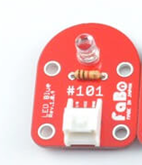
\includegraphics[width=\linewidth]{../../asset/image/text05-img026.png}
    \caption{LED}
  \end{minipage}
  %\hspace{0.01\columnwidth} % ここで隙間作成
  \begin{minipage}[t]{0.5\columnwidth}
    \centering
    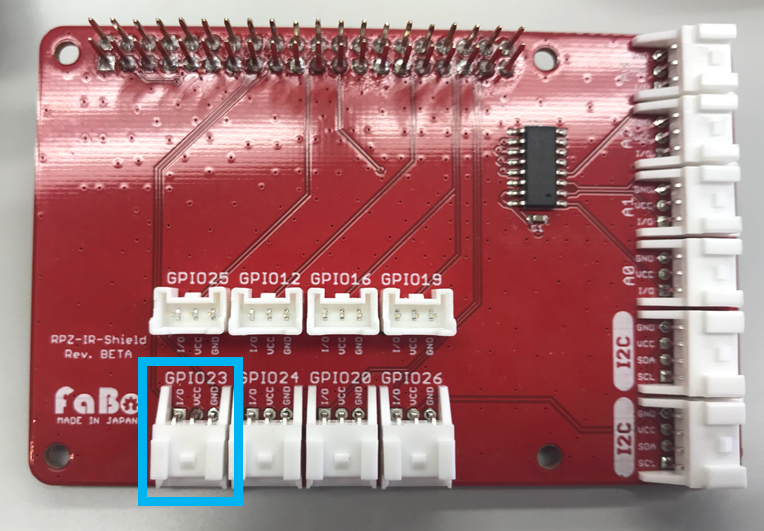
\includegraphics[width=\linewidth]{../../asset/image/text05-img027.png}
    \caption{GPIO23}
  \end{minipage}
\end{figure}

\begin{lstlisting}[caption=digout.hsp,label=digout.hsp]
#include "hsp3dish.as"
#include "rpz-gpio.as"

*main
	redraw 0
	font "",20
	pos 20,20
	mes "センサーが動いたり止まったりします"
	redraw 1

	gpio 23,1	<#blue#;GPIO23のブリックにONの信号を送る#>
	wait 100
	gpio 23,0	<#blue#;GPIO23のブリックにOFFの信号を送る#>
	wait 100
	goto *main
\end{lstlisting}

GPIO12,GPIO16,GPIO19,GPIO20,GPIO24,GPIO25,GPIO26はデジタル入出力装置用のピンです。センサーボードで使った\code{gpio}命令で使うことができます。\code{gpio GPIOピン番号,値}でブリックへの信号をONにしたりOFFにしたりすることができます。\\

digout.hspはデジタル出力装置用のプログラムです。LEDや\ruby{振動子}{しん|どう|し}に使うことができます。\\
\code{gpio GPIOピン番号,1}でブリックをONにします。\\
\code{gpio GPIOピン番号,0}でブリックをOFFにします。\\

\begin{tcolorbox}[title=\useOmetoi]
\begin{enumerate}
\addex{digout.hspのgpio 23,1をgpio 25,1に。gpio 23,0をgpio 25,0に変えましょう。LEDをGPIO25につけて、プログラムを実行しましょう。}
\addex{LEDを振動子(\#105)に変えて、digout.hspを実行しましょう。}
\end{enumerate}
\end{tcolorbox}

\end{document}
